%!TEX encoding = UTF-8 Unicode

%----------------------------------------------------------------------------------------
%	CHAPTER 3
%	Translator: SI(= Surgam Identidem)
%----------------------------------------------------------------------------------------

\chapterimage{chapter_head_1.pdf} % Chapter heading image






\chapter[Lie群]{Lie Group Theory\quad  Lie群}
\label{chap3}

\section*{本章概述}



\marginpar{
	
下面的图表是本章结构的示意图。 当你迷失方向的时候记得回来看看, 初学的时候不太需要看它。\sout{反正也看不懂}

\setlength{\unitlength}{0.8cm}
\begin{picture}(4, 3)\thicklines
\put(1.5, 1.8){\makebox(2.5, 1.2){\text{二维旋转}}}
\put(1, 0.7){\vector(1, 1){1.4}}
\put(4, 0.7){\vector(-1, 1){1.4}}
\put(0.5, 0.2){\makebox{$\mathcal{U}(1)$}}
\put(4, 0.2){\makebox{$\mathcal{SO}(2)$}}
\put(0, 0){\line(5, 0){5.5}}
\end{picture}

\begin{picture}(4, 3)\thicklines
\put(1.5, 1.8){\makebox(2.5, 1.2){\text{三维旋转}}}
\put(1, 0.7){\vector(1, 1){1.4}}
\put(4, 0.7){\vector(-1, 1){1.4}}
\put(0.5, 0.2){\makebox{$\mathcal{SU}(2)$}}
\put(4, 0.2){\makebox{$\mathcal{SO}(3)$}}
\put(0, 0){\line(5, 0){5.5}}
\end{picture}

\begin{picture}(5, 5)\thicklines
\put(1.5, 4){\makebox(2.5, 1.2){\text{Lorentz变换}}}
\put(2.5, 4.3){\vector(0, -1){0.8}}
\put(1.5, 2.5){\makebox(2.5, 1.2){ \text{Lie代数} $\hat{=} \, \mathfrak{su}(2) \oplus \mathfrak{su}(2) $  }}
\put(2.5, 2.8){\vector(0, -1){0.8}}
\put(1.5, 1){\makebox(2.5, 1.2){\text{双覆盖表示}}}
\put(0, 1){\line(5, 0){5.5}}
\end{picture}

\begin{picture}(5, 3)\thicklines
\put(1.5, 3){\makebox(2.5, 1.2){\text{Lorentz变换 + 平移}}}
\put(2.5, 3.2){\vector(0, -1){0.8}}
\put(1.5, 1.6){\makebox(2.5, 1.2){ \text{Poincare群} }}
\end{picture}

}

本章的最终目的是导出{\bf{Poincare群双覆盖的基本表示}}, 物理学现在认为Poincare群是时空根本的对称性群。 这些基本表示是描述所有基本粒子的必要工具, 每一种表示对应一种基本粒子, 它们揭示了自然界存在何种基本粒子。

我们从两个简单例子引出{\bf{群}}的定义, 然后作为学习Lie群理论的第一步, 我们讨论描述二维旋转变换的两种方式:
\begin{itemize}
	\item $2 \times 2$旋转矩阵。
	\item 单位复数。
\end{itemize}

接着我们尝试找出描述三维旋转的第二种方法(像复数那样, 当然第一种方法是$3\times3$矩阵), 第二法与一种超级重要的群 --- {\bf{$\mathcal{SU}(2)$}}。\mpar{$S$表示特殊(special), 它的含义为$\det (M) = 1$。 U表示幺正: $M^\dagger M = 1$, 数字$2$表示这个群起初是用$2 \times 2$矩阵定义的。}有关。 之后我们研究{\bf{Lie代数}}, 使用简便的Lie代数能够深入研究复杂的Lie群。 不同的群可以有相同的Lie代数, 但只有其中的一部分是基本的。 
从上述基础出发就能准确揭示自然的基本对称性群 --- Poincare群的双覆盖。 
%flag1:  double covers the Poincare group。 (Poincare 群的双覆盖) 翻译是否正确?
我们将利用已知的变换操作导出Lie代数, 并利用Lie代数得出不同的对称变换表示。 这样就能看出我们开始时使用的表示其实只是一种特殊情况。 这样我们又能研究Poincare群的重要部分 --- {\bf{Lorentz群}}, 我们会看到Lorentz群双覆盖的Lie代数由两份$\mathcal{SU}(2)$\, Lie代数所组成, 因此我们可以直接利用熟悉的$\mathcal{SU}(2)$群的结论。 最后我们将平移变换考虑进来, 这就是Poincare群, Poincare群就是Lorentz群加上平移。 完成上述所有之后我们终于可以将Poincare群双覆盖的基本表示进行分类, 这些在后面的章节中会大用特用, 我们将从中导出物理学的基本定律。

\section[群]{Groups\quad 群}
\label{sec3.1}
我们需要合适的数学工具描述对称性\sout{以和民科(贬义的)区分开}。 描述对称的数学分支称为{\bf{群论}}。 群论的一个分支{\bf{Lie理论}}\sout{谎言理论}描述连续的对称性, 物理中经常遇到这种情况。

我们把对称性定义为变换下的不变性, 而描述对称的群就定义为某些变换的集合。 让我们从两个简单例子开始体会群到底该怎么定义吧。



\begin{enumerate}
	\item 正方形是一些点的集合(例如四个顶点是该集合的一部分), 正方形的对称性是在某些变换下(变换: 将一个点映射到另一个点)保持不变的性质。
		
	符合条件的变换有绕中心旋转$90^\circ, 180^\circ, 270^\circ, 0^\circ$等等。 这些旋转操作将正方形映射到它自身。 我们称这个集合(正方形点集)在这样的变换下具有不变性。
	% flag1: This means they map every point of the set to a point that lies again in the set 没翻译, 因为觉得太啰嗦...
	
	\marginpar{
		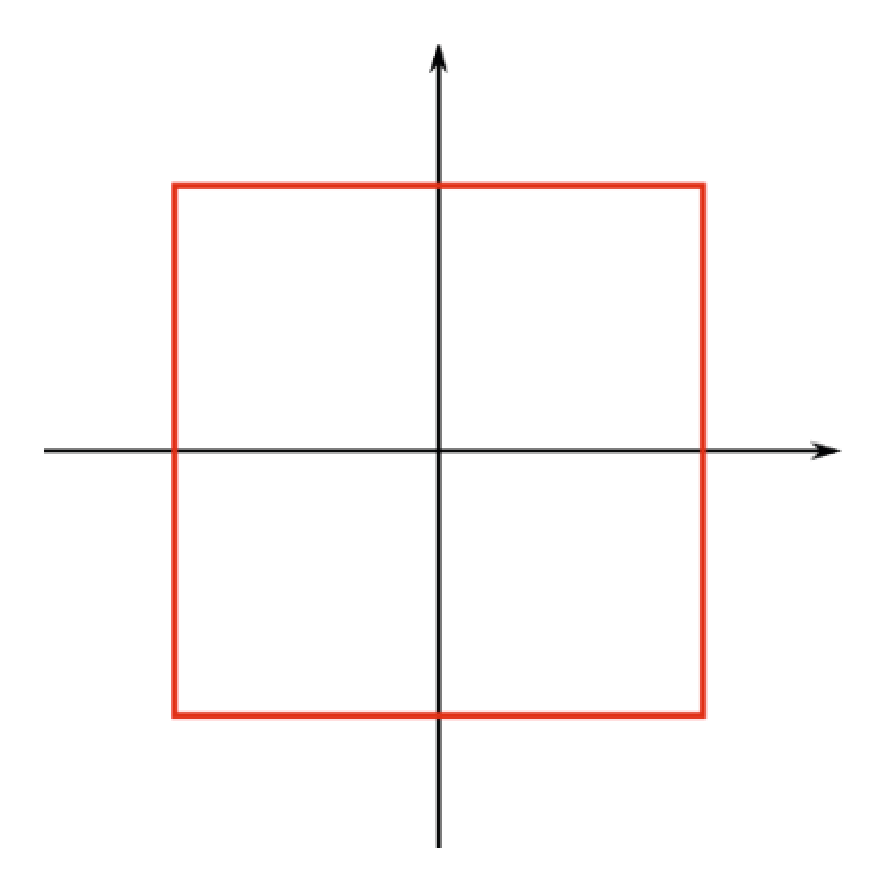
\includegraphics[scale=0.35]{fig3_1} 
		\figcaption{正方形}
	}
	
	\marginpar{
		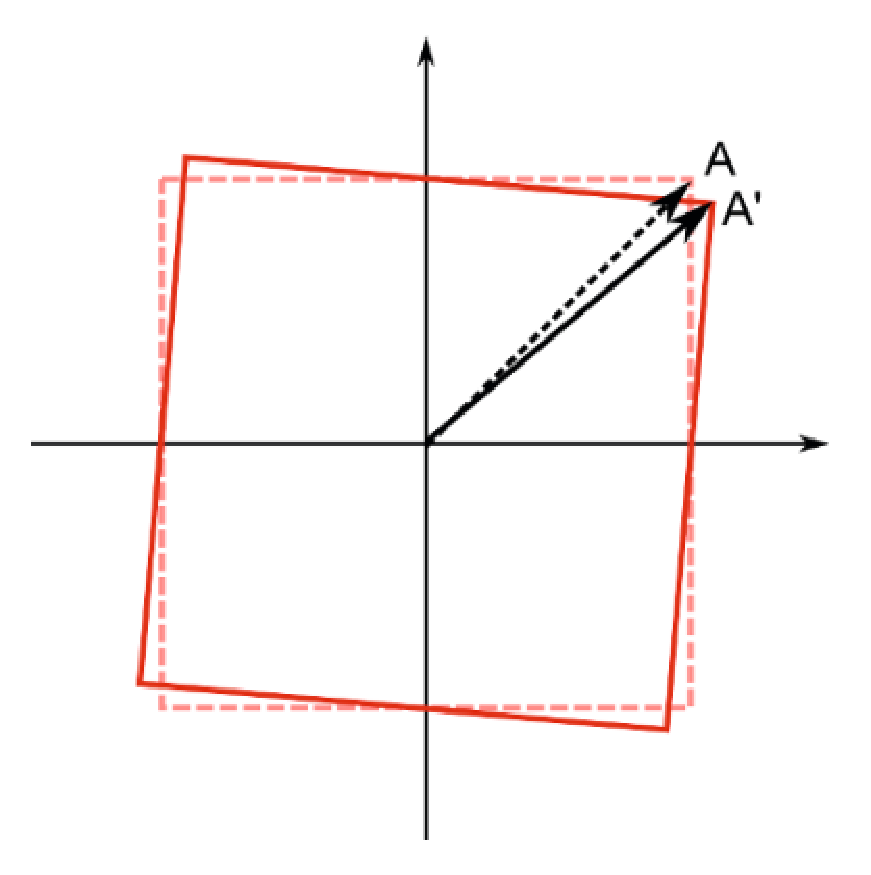
\includegraphics[scale=0.35]{fig3_2.eps}
		\figcaption{正方形绕中心顺时针旋转$5^\circ$}
	}
	
	注意不是所有旋转变换都对称。 我们关注顶点的变化就能看出来, 比如绕中心顺时针旋转$5^\circ$, 这个变换将顶点映射到原来正方形点集之外, 顶点$A$映射到了原来正方形集合之外的点$A'$。 因此这个旋转变换对正方形不具有对称性。 当然, 变换后的点集仍然是个正方形, 但却是不同的正方形(即不同点的集合)。 绕中心转$90^\circ$是对称的, 如图\ref{fig3.3}, 顶点$A$变换到点$B$, 等等, 原来的正方形点集变换到相同的集合。
	
	{
	\centering{
	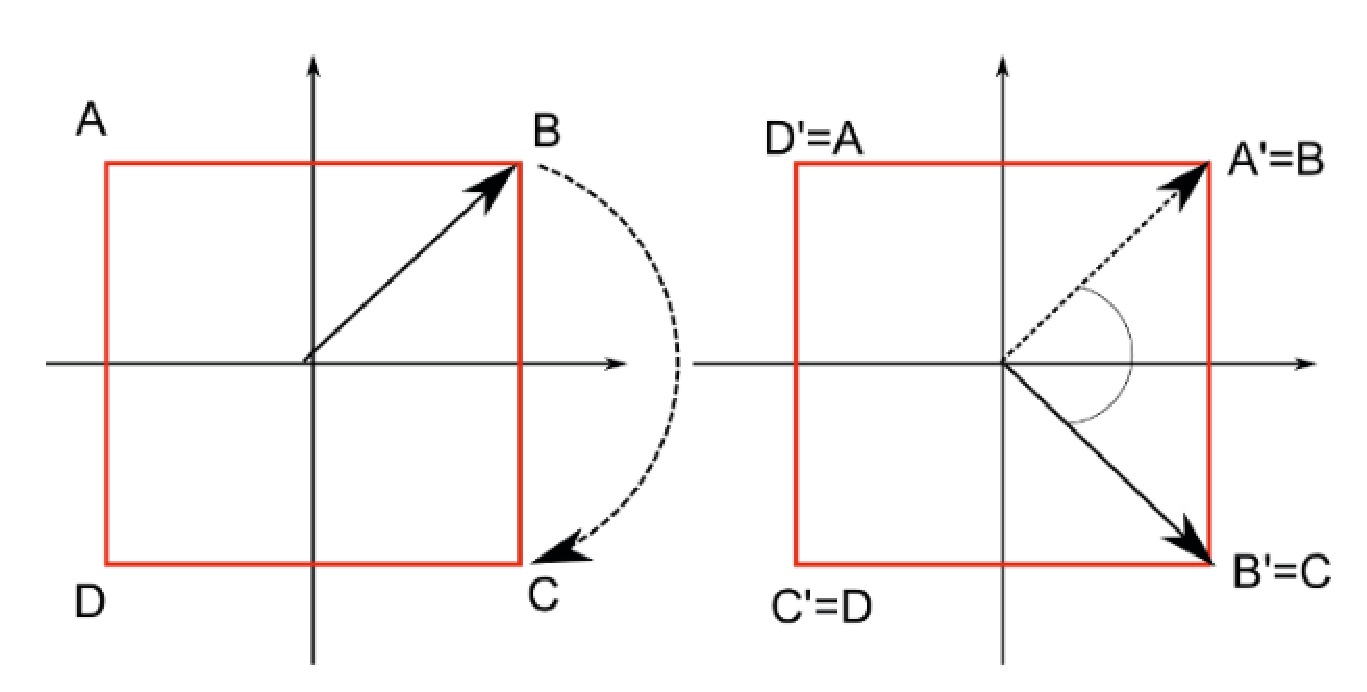
\includegraphics[scale=0.4]{fig3_3}
	\figcaption{正方形绕中心旋转$90^\circ$}
	\label{fig3.3}
	}}
	
	假如你看了一眼原来的正方形, 然后闭上眼睛, 这时有人把正方形做了一个变换。 如果你不能分辨这个正方形是否发生变化, 那么这个变换就是个对称变换。
	
	我们把所有使正方形不变的变换构成的集合称为群。 变换参数(本例中就是旋转角度)不能任意取值(而是取分立的数), 这个群称为离散群。
	
	\item 另一个例子是使单位圆不变的变换构成的集合。 类似地, 单位圆还是一些点构成的集合, 对称变换把这个集合映射到它自身。
	
	单位圆绕圆心旋转任意角度都不变。 换言之, 变换参数(这里就是旋转角度)可以取任意值, 因此这个群称为连续群。
\end{enumerate}
	\marginpar{
		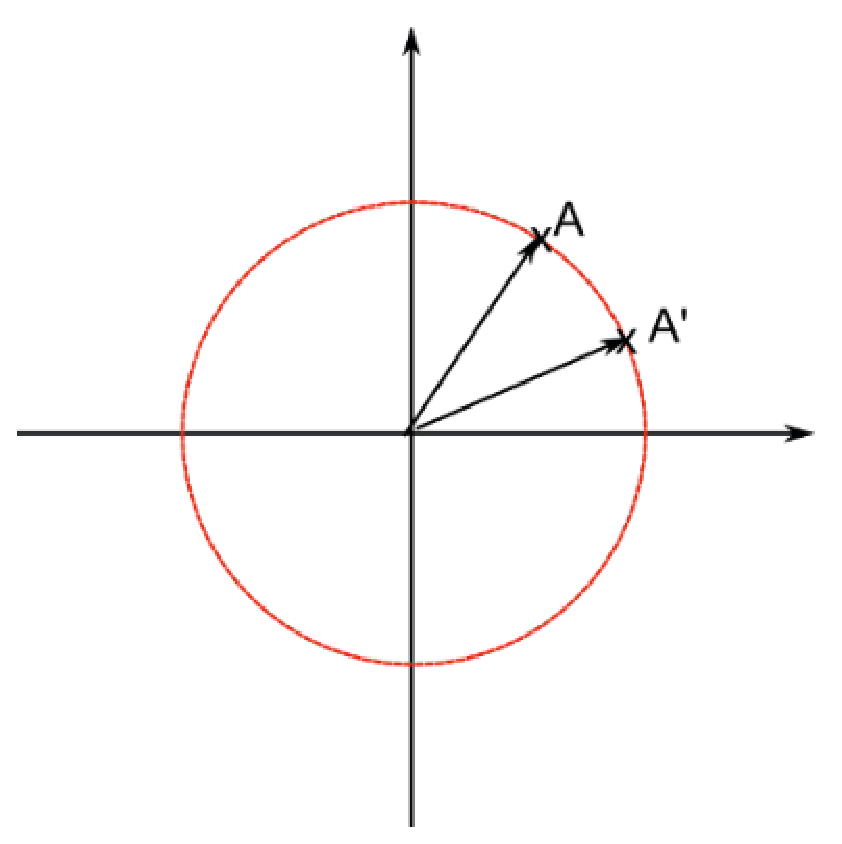
\includegraphics[scale=0.35]{fig3_4.eps}
		\figcaption{单位圆绕圆心旋转任意角度都不变}
	}

数学中除了几何图形之外还有好多别的都有对称性。 例如,对于向量, 我们可以考虑所有让向量长度不变的变换构成的集合。 看出本节开头对称性定义的普遍性了没? 对称性就是变换下的不变性。 非常幸运, 搞数学的早已建立了群论, 它可以研究所有类型的对称性\mpar{历史上数学家们建立群论最初是为了描述方程的对称性}。

为了让精确描述对称性的工具 --- 群的定义来的自然一点, 我们把对称性的定义用数学语言精炼一下:
\begin{itemize}
	\item 对某物什么也不做(比如转个$0^\circ$)当然也是对称变换(按照我们的对称性定义), 因此任何群都需要包含一个恒等变换(恒等元)。 在上面的例子里, 恒等元就是旋转$0^\circ$。
	
	\item 对某物先做变换再做逆变换的结果必须等于啥也不做。 因此对于群中的任意元素(简称群元), 必须有相应的逆元素。 按定义, 先做变换再做逆变换等于恒等变换。 例如先转$90^\circ$再转$-90^\circ$(先逆针再顺针转)与旋转$0^\circ$相同。
	
	\item 先做一个对称变换再做一个对称变换, 总体效果必须还是对称变换。 例如先旋转$90^\circ$再转$180^\circ$等于直接转$270^\circ$, 后者也是对称变换。 对称变换的这个性质称为封闭性。
	
	\item 对称变换之间必须满足结合律。 例如先转$90^\circ$再转$40^\circ$再转$110^\circ$与先转$130^\circ$再转$110^\circ$相同, 先转$90^\circ$再转$150^\circ$也一样。 用符号表示更加清楚:
	\begin{equation}\label{equ3.1}
	R(110^\circ) R(40^\circ) R(90^\circ) = R(110^\circ)\bigg( R(40^\circ)R(90^\circ) \bigg) = R(110^\circ) R(130^\circ)
	\end{equation}
	\begin{equation}\label{equ3.2}
	R(110^\circ) R(40^\circ) R(90^\circ) = \bigg( R(110^\circ) R(40^\circ) \bigg) R(90^\circ) = R(150^\circ) R(90^\circ)
	\end{equation}
	这个性质称为{\bf 结合律}。
	
	\item 我们要有规定两个群元(对称变换)怎样合体的规则, 它是个{\bf 二元运算}(两个群元合体成一个), 我们称它为{\bf 群乘法}。 
	
	在上面的例子里, 旋转变换的标准表示方法是用旋转矩阵\mpar{旋转矩阵见附录A.2.}, 两个群元(两个旋转矩阵, 或两个旋转操作)合体的规则是线性代数里的矩阵乘法。 同样的变换经常有不同的表示方法\mpar{例如, 二维平面旋转还可以用单位复数描述, 相应的群乘法是复数乘法。 稍后就讨论这一点。}, 群论非常系统性地概括了所有形式。 群论的分支 --- {\bf 表示论}就是研究相同变换的不同描述方式的, 我们在\ref{sec3.5}节学习表示论。
\end{itemize}

\ 

我们把上述群与对称变换的特征用严谨的数学语言表达, 再将它们提升为公理, 满足这些公理的数学结构就是一个群。 数学系的群论书可能更喜欢在开头就从天上掉下来这些公理。 必须指出满足群公理的结构可能是超级抽象的, 但我们现在只关注上面例子里的旋转变换那样的群。 \sout{因为我们是物理系的, 而且这是本物理书}

\ 

(我们通过对称变换的性质导出的)群公理\mpar{别担心怎么才能根据这些公理凑出一个群来。 搞物理的往往是从某个变换出发, 考察它是否符合群公理, 如果是\sout{经常是}那么就可以应用群论来解决问题。}: 

一个群就是一个集合$G$加上一个定义在$G$上的二元运算(群乘法)$\circ$, 当然$(G, \circ)$还要满足以下公理: 
\begin{itemize}
	\item 封闭性: 对于任意$g_1, g_2 \in G, g_1 \circ g_2 \in G$
	
	\item 单位元: 存在单位元$e \in G$使得对于所有$g \in G, g\circ e = g = e \circ g$
	
	\item 逆元: 对于任意$g \in G$, 存在相应的逆元$g^{-1} \in G$使得$g \circ g^{-1} = e = g^{-1} \circ g$
	
	\item 结合律: 对于任意$g_1, g_2, g_3 \in G, g_1 \circ (g_2 \circ g_3) = (g_1 \circ g_2) \circ g_3$ 
\end{itemize}

总结: 某物体在一些变换下保持不变, 这些变换组成\footnote{我在想这里该用`构成'还是`组成', 后来我觉得无所谓, 因为这不是初中化学...(分子构成物质, 元素组成物质...) --- 译者(SI)}的集合叫做对称群。 对于Minkowski时空, Minkowski度规\mpar{复习一下, Minkowski度规就是在Minkowski空间中用来计算距离和长度的工具, 见第二章。}在变换下保持不变, 相应的对称群称为Poincare群。

要注意群的定义完全与变换的物体是啥没有关系。 我们可以脱离特定物体而只研究对称变换本身, 群的定义将变换从物体中`提取'出来了。 这是非常有用的, 许多不同事物具有同样或同类的对称性。 群论让我们不用管变换的物体(圆还是正方形), 只研究变换(例如旋转)的普遍性质。


\section[二维旋转]{Rotations in two Dimensions\quad 二维旋转}
\label{sec3.2}
我们从一个简单而重要的例子开始学习群论。考虑那些让二维平面中的向量长度不变的对称变换。符合条件的有旋转和反射\mpar{当然还有平移。平移的数学描述与前两者有些不同,我们之后再讨论它。}。它们也是圆的对称变换,一个单位元旋转或反射之后还是单位圆。可见同一个群(对应一种变换)可以作用于不同类物体:圆(几何图形),或者向量。本节考虑向量,可以用旋转矩阵表示向量的旋转或反射,\mpar{旋转矩阵的推导见附录A.2.},将起点位于原点的向量绕原点逆时针旋转$\theta$角度的旋转矩阵为:
\begin{equation}
\label{equ3.3}
R_\theta = 
	\begin{pmatrix}
		\cos \theta & \sin \theta \\
		-\sin \theta & \cos \theta
	\end{pmatrix}
\end{equation}

关于$x$轴与$y$轴的反射变换用矩阵表示为:
\begin{equation}
\label{equ3.4}
P_x = 	\begin{pmatrix}
			-1 & 0 \\ 0 & 1
		\end{pmatrix}
\quad
P_y = 	\begin{pmatrix}
			1 & 0 \\ 0 & -1
		\end{pmatrix}
\end{equation}
将矩阵乘法作为群乘法$\circ$, 可以验证$R(\theta), P_x, P_y$与矩阵乘法符合群公理,因而构成一个群,亦即旋转与反射变换构成一个群。

可以用更抽象的方式表达‘所有让二维向量长度不变的变换’,向量长度就是向量与自身点乘的平方根($|a| = \sqrt{a \cdot a}$). 向量长度在变换$a \rightarrow a'$下不变意味着\footnote{等号上面的!只是起强调、提示作用 --- 译者(SI)}:
\begin{equation}
\label{equ3.5}
a' \cdot a' \stackrel{!}{=} a \cdot a
\end{equation}

将变换矩阵记作$\mathcal{O}$,变换即为$a \rightarrow a' = \mathcal{O}a$.
\begin{equation}
\label{equ3.6}
a \cdot a = a^{\mathrm{T}} a \rightarrow a'^{\mathrm{T}} a' = (\mathcal{O} a)^{\mathrm{T}} \mathcal{O} a = a^{\mathrm{T}} \mathcal{O}^{\mathrm{T}} \mathcal{O} a \stackrel{!}{=} a^{\mathrm{T}} a = a \cdot a
\end{equation}
由此可见,使向量长度不变的变换必须满足:
\begin{equation}
\label{equ3.7}
\mathcal{O}^{\mathrm{T}} \mathcal{O} = I
\end{equation}
其中$I$表示单位矩阵\mpar{ I = 
	\[\begin{pmatrix}
		1 & 0 \\ 0 & 1
	\end{pmatrix}\]}。前文的旋转和反射矩阵都满足此条件\mpar{例如\ref{equ3.3}式的矩阵,
	$R_\theta^{\mathrm{T}} R = 
	\begin{pmatrix}
		\cos \theta & -\sin \theta \\
		\sin \theta & \cos \theta
	\end{pmatrix}
	\begin{pmatrix}
		\cos \theta & \sin \theta \\
		-\sin \theta & \cos \theta
	\end{pmatrix}
	 = 
	 \begin{pmatrix}
		 \cos^2 \theta + \sin^2 \theta & 0 \\
		 0 & \sin^2 \theta + \cos^2 \theta
	 \end{pmatrix}
	 =
	 \begin{pmatrix}
		 1 & 0 \\ 0 & 1
	 \end{pmatrix}
	$
}%mpar
$2 \times 2$矩阵中所有满足\ref{equ3.7}式的矩阵构成了$\mathcal{O}(2)$群,即所有$2 \times 2$正交矩阵构成的群\mpar{严谨地说,任意$2 \times 2$正交矩阵可以表示为\ref{equ3.3}、\ref{equ3.4}式,或者它们的乘积的形式。}。我们可以找出这个群中描述旋转变换的那一部分(构成一个子群)。根据\ref{equ3.7}式:
\begin{align}
\det(\mathcal{O}^{\mathrm{T}} O ) = \det(O^{\mathrm{T}}) \det(O) \stackrel{!}{=} \det(I) = 1 \nonumber\\
\label{equ3.8}
(\det(\mathcal{O}))^2 \stackrel{!}{=} 1 \rightarrow \det{(\mathcal{O})} \stackrel{!}{=} \pm 1
\end{align}

$\det \mathcal{O} = 1$的矩阵对应旋转变换\mpar{见\ref{equ3.3}与\ref{equ3.4}式。反射矩阵的行列式等于$-1$。}

条件
\begin{align}
\label{equ3.9}
\mathcal{O}^{\mathrm{T}} \mathcal{O} = I \\
\label{equ3.10}
\det \mathcal{O} = 1
\end{align}
定义了$\mathcal{SO}(2)$群,`$\mathcal{S}$'表示‘特殊’(special),`$\mathcal{O}$'表示‘正交’(orthogonal)。

$\mathcal{SO}(2)$包含的旋转变换保持了坐标系的取向,即一个右手坐标系\mpar{右手坐标系与左手坐标系见附录A.5.}经旋转变换后还是右手系,而反射变换会改变它的取向。用线性代数的概念来说,我们规定$\mathcal{SO}(2)$中的矩阵行列式必须为$+1$。

\subsection[单位复数表示旋转变换]{Rotations with Unit Complex Numbers\quad 单位复数表示旋转变换}
\label{sec3.2.1}
还可以用单位复数来表示旋转变换:向量绕原点旋转$\theta$角可以表示为用单位复数$z$乘此向量(单位复数意为$z = a + ib$,$|z|^2 = z^* z = 1$)\mpar{上标$ ^*$表示复数的共轭复数:$z = a + ib \rightarrow z^* = a - ib$}。

所有单位复数构成一个群,称为$\mathcal{U}(1)$,群乘法即为复数乘法,不难验证它符合群公理。为了看出它与之前引入的$\mathcal{O}(3), \mathcal{SO}(3)$群的关系,我们将$\mathcal{U}(1)$群的条件 --- 单位复数表示为\mpar{定义中包含复数乘法的群的普遍性质见\ref{sec3.10}节的附录。}, $\forall \mathcal{U} \in \mathcal{U}(1)$:
\begin{equation}
\label{equ3.11}
\mathcal{U}^* \mathcal{U} = 1
\end{equation}
单位复数另一种形式是利用欧拉公式\mpar{附录B.4.2推导了传说中的欧拉公式。对任意复数$z = a + ib$, $a$称为$z$的实部,记为$\Re(z) = a$; $b$称为虚部,记为$\Im(z) = b$. 欧拉公式中$R_\theta$的实部为$\cos  \theta$, 虚部为$\sin \theta$.}:% Euler翻译为欧拉
\begin{equation}
\label{equ3.12}
R_\theta = \mathrm{e}^{i\,\theta} = \cos \theta + i\sin \theta
\end{equation}
$R(\theta)$的模(长度)为:
\begin{equation}
\label{equ3.13}
R_\theta^* R_\theta = \mathrm{e}^{-i\,\theta} \mathrm{e}^{i\,\theta} = \big( \cos \theta - i \sin \theta  \big) \big( \cos \theta + i \sin \theta \big) = 1
\end{equation}

\marginpar{
	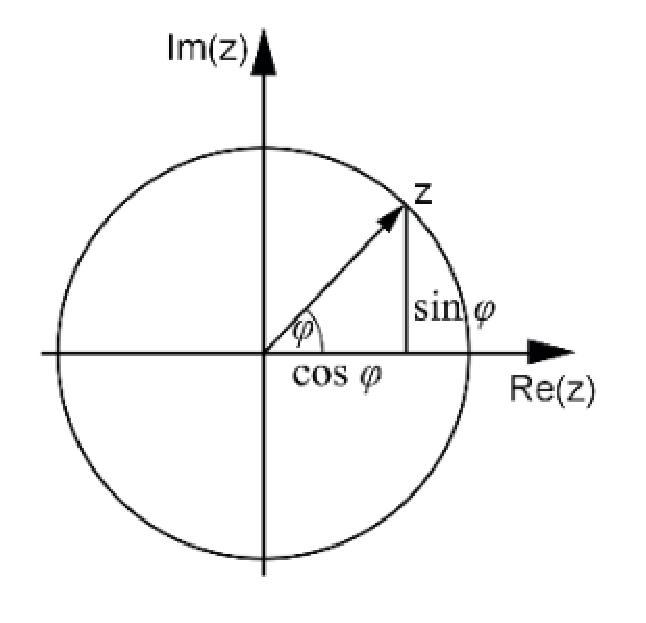
\includegraphics[scale=0.45]{fig3_5.eps} 
	\figcaption{单位复数在复平面的单位圆上}
	}

例:将向量$(3,  5)$旋转$90^\circ$:
\begin{equation}
\label{equ3.14}
z \rightarrow z' = \mathrm{e}^{i\, 90^\circ}z = \bigg( \underbrace{\cos 90^\circ}_{=0} + i\underbrace{\sin 90^\circ}_{=1} \bigg) (3 + 5i) = i(3 + 5i) = 3i - 5
\end{equation}

图3.6绘制了旋转前后的向量(复数),图中可见复数乘以$\mathrm{e}^{i\, 90^\circ}$旋转了$90^\circ$.
\marginpar{
	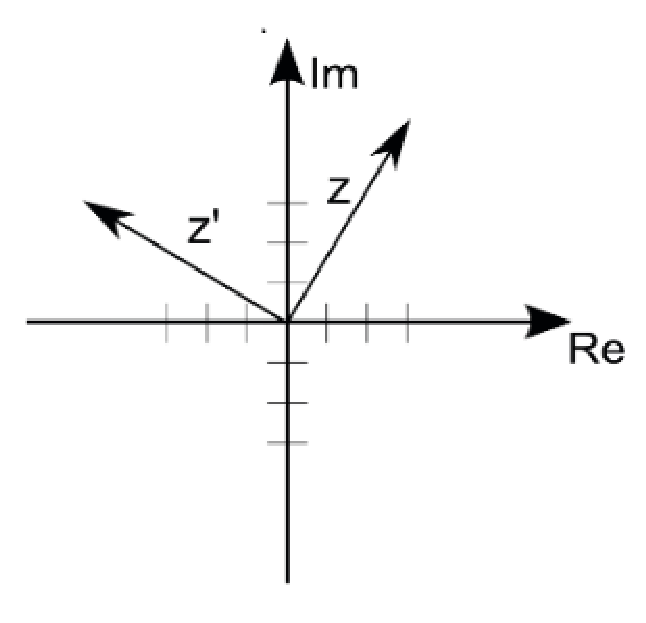
\includegraphics[scale=0.45]{fig3_6.eps} 
	\figcaption{复数通过乘以单位复数进行旋转}
	}
需要注意$\mathrm{e}^{i\, 90^\circ}$作用于(乘以)向量对应的复数而非向量本身。描述二维旋转只需要一个参数:旋转角$\phi$. 而复数有两个自由度(实部和虚部),因此我们加上单位复数的限制:$|z| = \text{实部}^2 + \text{虚部}^2 = 1$,只剩一个自由度。

描述二维旋转的两种方式 --- 单位复数与$2 \times 2$矩阵(矩阵元都是实数)通过如下方式关联。定义:
\begin{equation}
\label{equ3.15}
\mathbf{1} = 
	\begin{pmatrix}
		1 & 0 \\ 0 & 1
	\end{pmatrix}
,\quad
\mathbf{i} = 
	\begin{pmatrix}
		0 & -1 \\ 1 & 0
	\end{pmatrix}
\end{equation}
不难验证这样定义的$\mathbf{1, i}$仍然满足:
\begin{equation}
\mathbf{1}^2 = \mathbf{1},\quad \mathbf{i}^2 = -\mathbf{1},\quad \mathbf{1i} = \mathbf{i1} = \mathbf{i}
\end{equation}
这样单位复数对应的$2 \times 2$实数矩阵为\footnote{原文此式有误,译文已参照勘误表修改。}
\begin{equation}
\label{equ3.17}
R_\theta = \cos \theta + i\sin\theta = \cos \theta 
\begin{pmatrix}
	1 & 0 \\ 0 & 1
\end{pmatrix}
+ \sin \theta
\begin{pmatrix}
	0 & -1 \\ 1 & 0
\end{pmatrix}
=
\begin{pmatrix}
	\cos \theta & -\sin \theta \\
	\sin \theta & \cos \theta
\end{pmatrix}
\end{equation}
可见,定义了复单位$i \rightarrow \text{实矩阵}$的对应关系后,单位复数就回到了熟悉的旋转矩阵。还有一点要注意:旋转矩阵作用于向量(列矩阵),而我们将$i$与$2 \times 2$矩阵相联系,因此被旋转的向量(与一个复数对应)也将变成一个$2 \times 2$矩阵。

例:任意向量$(a, b)$对应的复数对应的$2 \times 2$矩阵为:
\begin{equation}
\label{equ3.18}
z = a + ib = a
\begin{pmatrix}
	1 & 0 \\ 0 & 1
\end{pmatrix}
+ b
\begin{pmatrix}
	0 & -1 \\ 1 & 0
\end{pmatrix}
=
\begin{pmatrix}
	a & -b \\ b & a
\end{pmatrix}
\end{equation}
将旋转矩阵作用于$z$:
\begin{eqnarray}
\label{sec3.19}
	z' &=& \begin{pmatrix}
			a' & -b' \\ b' & a'
		 \end{pmatrix}
	= R_\theta z = 
		\begin{pmatrix}
			\cos \theta & -\sin \theta \\
			\sin \theta & \cos \theta
		\end{pmatrix}
		\begin{pmatrix}
			a & -b \\ b & a
		\end{pmatrix}
	\nonumber \\
	&=& \begin{pmatrix}
			a\cos\theta - b\sin \theta & - b\cos \theta - a \sin \theta \\
			a\sin \theta + b\cos \theta & -b \sin \theta + a \cos \theta
		\end{pmatrix}
\end{eqnarray}
由上式可得
\begin{align}
\label{equ3.20}
a' &= a \cos \theta - b \sin \theta \\
\label{equ3.21}
b' &= a \sin \theta + b \cos \theta
\end{align}
这与旋转矩阵作用于向量(列矩阵形式)相同:
\begin{equation}
\label{equ3.22}
	\begin{pmatrix}
		\cos \theta & -\sin \theta \\
		\sin \theta & \cos \theta
	\end{pmatrix}
	\begin{pmatrix}
		a \\ b
	\end{pmatrix}
	=
	\begin{pmatrix}
		a \cos \theta - b \sin \theta \\
		a \sin \theta + b \cos \theta
	\end{pmatrix}
	=
	\begin{pmatrix}
		a' \\ b'
	\end{pmatrix}
\end{equation}
我们看到这两种表示方法是一回事儿,用数学术语来说,$\mathcal{SO}(2)$与$\mathcal{U}(1)$间有一个同构映射\mpar{如果映射$\Pi: G \rightarrow G'$是一一映射,并且满足:$\forall g_1, g_2 \in G, \Pi(g_1) \circ \Pi(g_2) = \Pi(g_1 \circ g_2)$, 则$\Pi$就是同构映射,并且称群$G, G'$是同构的。}。这一点太重要了,之后的篇幅会不断出现这种思想。

下面研究三维旋转,尝试找出它的两种描述方法。

\section[三维旋转]{Rotations in three Dimensions\quad 三维旋转}
\label{sec3.3}
三维空间向量旋转变换当然可以用$3 \times 3$旋转矩阵\footnote{原文公式有误,译文已按勘误表改正。}:
\begin{align}
R_x =
	\begin{pmatrix}
		1 & 0 & 0 \\
		0 & \cos \theta & -\sin \theta \\
		0 & \sin \theta & \cos \theta
	\end{pmatrix}
\quad
R_y = 
	\begin{pmatrix}
		\cos \theta & 0 & \sin \theta \\
		0 & 1 & 0 \\
		-\sin \theta & 0 & \cos \theta
	\end{pmatrix}
\nonumber \\
\label{equ3.23}
R_z =
	\begin{pmatrix}
		\cos \theta & -\sin \theta & 0 \\
		\sin \theta & \cos \theta & 0 \\
		0 & 0 & 1
	\end{pmatrix}
\end{align}
类比$\mathcal{SO}(2)$群,上面三个矩阵构成了$\mathcal{SO}(3)$群的一组基\mpar{基的概念见附录A.1.}。这意味着$\mathcal{SO}(3)$中的任意群元(矩阵)都可以写为$R_x, R_y, R_z$的线性组合,且系数唯一。
将向量
\begin{equation*}
\vec{v} = \begin{pmatrix}
			1 \\ 0 \\ 0
		\end{pmatrix}
\end{equation*}
绕$z$轴旋转\mpar{三维向量旋转的一般情况的推导见附录A.2.}就是用旋转矩阵乘以向量:
\begin{equation}
\label{equ3.24}
R_z(\theta) \vec{v} = 
	\begin{pmatrix}
		\cos \theta & -\sin \theta & 0 \\
		\sin \theta & \cos \theta & 0 \\
		0 & 0 & 1
	\end{pmatrix}
	\begin{pmatrix}
		1 \\ 0 \\ 0
	\end{pmatrix}
=
	\begin{pmatrix}
		\cos \theta \\ \sin \theta \\ 0
	\end{pmatrix}
\end{equation}
为找出描述三维旋转的第二法,我们尝试把复数的概念扩展到三维空间。首先试着把$2$维的复数(实部虚部两个自由度)扩展为$3$维复数,但前人探索发现没有$3$维的,但存在$4$维‘复数’,称为{\bf 四元数(quaternions)}。下面就会看到四元数正是描述三维旋转的第二法,并且它还能深刻揭示宇宙 --- 四维时空的规律。描述三维旋转需要三个参数(绕$x,y,z$轴的旋转角),而四元数有四个参数,这与二维旋转的情况类似\mpar{单位复数描述二维旋转。}。四元数加上单位长度的限制 ---单位四元数(三个自由参数)能够描述三维旋转。

\subsection[四元数]{Quaternions\quad 四元数}
\label{sec3.3.1}
我们类比复数来构造四元数,复数只有一个虚单位$i$,而四元数里定义三个虚单位,记作$\mathbf{i,j,k}$,它们仍然满足
\begin{equation}
\label{equ3.25}
\mathbf{i}^2 = \mathbf{j}^2 = \mathbf{k}^2 = -1
\end{equation}
这样任意一个四元数$q$表示为
\begin{equation}
\label{equ3.26}
q = a\mathbf{1} + b\mathbf{i} + c\mathbf{j} + d\mathbf{k}
\end{equation}
其中$a, b, c, d \in \mathbb{R}$, $\mathbf{1}$就是正常的实数1。\footnote{$\mathbf{1,i,j,k}$用黑体表示是为了强调它们是四元数的基。---译者(SI)}

要想定义四元数间的乘法,必须定义虚单位间的乘法规则,比如$\mathbf{ij} = ?$. 为此再定义
\begin{equation}
\label{equ3.27}
\mathbf{ijk} = -1
\end{equation}
这样虚单位间的乘法就没问题了,例如,为导出$\mathbf{ij} = \mathbf{k}$, 在\ref{equ3.27}式等号两侧右乘$\mathbf{k}$:
\begin{equation}
\label{equ3.28}
\mathbf{ij} \underbrace{\mathbf{kk}}_{= -1} = -\mathbf{k} \rightarrow \mathbf{ij} = \mathbf{k}
\end{equation}

单位四元数$q = a\mathbf{1} + b\mathbf{i} + c\mathbf{j} + d\mathbf{k}$满足\mpar{符号$\dag$称为`dagger',表示转置加取复共轭,即$a^\dag = (a^*)^T$。实数向量间的点乘定义为$a \cdot b = a^T b$, 向量用列矩阵表示,其转置为行矩阵,于是点乘的定义符合矩阵乘法规则。四元数对应的列矩阵含复数,为使四元数与它自身相乘结果为实数(实数结果可表示‘长度’),在转置之外还加上取复共轭。}:
\begin{align}
q^\dag q &\stackrel{!}{=} 1 \nonumber\\
\label{equ3.29}
\rightarrow (a\mathbf{1} - b\mathbf{i} - c\mathbf{j} - d\mathbf{k}) (a\mathbf{1} +& b\mathbf{i} + c\mathbf{j} + d\mathbf{k}) = a^2 + b^2 + c^2 + d^2 \stackrel{!}{=} 1
\end{align}

就像单位复数构成一个群(群乘法为复数乘法)那样,单位四元数也构成一个群(群乘法为四元数乘法)。

类似于我们将二维复数与$2 \times 2$实数矩阵建立联系的做法,四元数也可如此 --- 将四个基$\mathbf{1,i,j,k}$与合适的矩阵一一对应。其中一种方法(还有别的方式)是将它们与$2 \times 2$复数矩阵对应:
\begin{align}
\mathbf{1} = \begin{pmatrix}
				1 & 0 \\ 0 & 1
			 \end{pmatrix}
\quad &, \quad
\mathbf{i} = \begin{pmatrix}
				0 & 1 \\ -1 & 0 
			 \end{pmatrix}
\nonumber \\
\label{equ3.30}
\mathbf{j} = \begin{pmatrix}
				0 & -i \\ -i & 0
			 \end{pmatrix}
\quad &, \quad
\mathbf{k} = \begin{pmatrix}
				i & 0 \\
				0 & -i
			 \end{pmatrix}
\end{align}
不难验证上式满足四元数乘法,比如\ref{equ3.25}、\ref{equ3.27}式。这样任意一个四元数都可用矩阵表示为:
\begin{equation}
\label{equ3.31}
q = a\mathbf{1} + b\mathbf{i} + c\mathbf{j} + d\mathbf{k} = \begin{pmatrix}
	a + di & -b - ci \\
	b - ci & a - di
	\end{pmatrix}
\end{equation}
由上式可见
\begin{equation}
\label{equ3.32}
\det(q) = a^2 + b^2 + c^2 + d^2
\end{equation}
上式与\ref{equ3.29}式比较可以发现单位四元数对应的矩阵的行列式为$1$。因此单位四元数对应的$2 \times 2$复数矩阵$\mathcal{U}$满足:
\begin{equation}
\label{equ3.33}
\mathcal{U}^\dag \mathcal{U} = 1, \quad \text{且} \det(\mathcal{U}) = 1
\end{equation}
注意\ref{equ3.30}式中的矩阵是线性独立的\mpar{线性独立的概念见附录A.1.},它们构成群$\mathcal{SU}(2)$的基。与之前相同,$\mathcal{S}$表示特殊(special),含义为$\det (\mathcal{U}) = 1$;$\mathcal{U}$表示幺正(unitary)\mpar{进一步介绍见本章附录 --- \ref{sec3.10}节。},即$\mathcal{U}^\dag \mathcal{U} = 1$。任意单位四元数都唯一对应$\mathcal{SU}(2)$群中的一个群元。

$\mathcal{SU}(2)$群如何与三维旋转联系?事情正在起变化,$\mathcal{SU}(2)$群与$\mathcal{SO}(3)$\mpar{$\mathcal{SO}(3)$群就是三维旋转矩阵构成的群。}之间的对应关系并不像二维旋转中$\mathcal{U}(1)$与$\mathcal{SO}(2)$那样简单。

2维虚数$z = a + ib$与2维向量很容易对应。单位复数保证了矢量长度在旋转变换下不变\mpar{注意这里的$R$表示一个单位复数,即$R^* R = 1$, $R$与复数$z$相乘就将$z$进行旋转变换。}:$(Rz)^* Rz = z^* R^* Rz = z^* z$。四元数有$4$个参数,它与三维向量的对应关系是并不明显。我们尝试将三维向量$\vec{v} = (x, y, z)$定义为如下四元数\footnote{注意下式中的$\mathbf{ijk}$是四元数的‘基’而非三维直角坐标系的基矢。 --- 译者}:
\begin{equation}
\label{equ3.34}
v \equiv x\mathbf{i} + y\mathbf{j} + z\mathbf{k}
\end{equation}
利用前述四元数的矩阵表示可得:
\begin{equation}
\label{equ3.35}
\det(v) = x^2 + y^2 + z^2
\end{equation}
于是保持向量$(x, y, z)$长度不变的变换就对应于保持矩阵行列式不变的矩阵变换。而{\bf 单位}四元数对应矩阵都具有{\bf 单位}行列式,它与任意矩阵相乘不改变该矩阵的行列式\footnote{利用$\det(AB) = \det(A)\det(B)$, --- 译者}。进展很顺利,但现在有个微妙的状况:继续猜想下去,我们会认为用单位四元数$u$旋转向量(对应的四元数)$v$直接用$u$乘以$v$就可以了(按照四元数乘法规则)。但细想起来这却不行,因为根据\ref{equ3.34}式,我们把任意三维向量对应的四元数定义在$\mathbb{R}\mathbf{i} + \mathbb{R}\mathbf{j} + \mathbb{R}\mathbf{k}$的范围内,$u$与$v$的四元数乘积会超出这个范围,这样向量旋转后可能不是个向量!这当然不行。

事实上,旋转变换表示为:
\begin{equation}
\label{equ3.36}
v' = q^{-1} v q
\end{equation}
其中$v$, $v'$分别为旋转前后的向量,$q$为表示旋转的单位四元数。

这样我们终于实现了描述三维旋转的第二法 --- 单位四元数。

例:定义$u$是$\mathbb{R}\mathbf{i} + \mathbb{R}\mathbf{j} + \mathbb{R}\mathbf{k}$中的某一单位向量,则任意单位四元数$t$可表示为:
\begin{equation}
\label{equ3.37}
t = \cos \theta +  u\sin \theta
\end{equation}
利用\ref{equ3.34}式,任意三维向量$\vec{v}$可表示为:
\begin{equation}
\label{equ3.38}
\vec{v} = (v_x, v_y, v_z)^T = v_x \mathbf{i} + v_y \mathbf{j} + v_z \mathbf{k} \underbrace{=}_{\ref{equ3.31}\text{式}} \begin{pmatrix}
		iv_z & -v_x - iv_y \\
		v_x - iv_y & -iv_z
	\end{pmatrix}
\end{equation}

简明起见我们举个特例,把向量$\vec{v} = (1, 0, 0)^T$绕$z$轴旋转。
\begin{align}
\label{equ3.39}
\vec{v} &= (1, 0, 0)^T \rightarrow v = 1\mathbf{i} + 0\mathbf{j} + 0\mathbf{k} = 
	\begin{pmatrix}
		0 & -1 \\ 1 & 0
	\end{pmatrix}
\\
\label{equ3.40}
R_z(\theta) &= \cos \theta \mathbf{1} + \sin \theta \mathbf{k} =
	\begin{pmatrix}
		\cos \theta + i\sin \theta & 0 \\
		0 & \cos \theta - i\sin \theta
	\end{pmatrix}
\end{align}
上式也可用欧拉公式写出\mpar{欧拉公式的推导见附录B.4.2}:
\begin{equation}
\label{equ3.41}
\mathrm{e}^{ix} = \cos x + i\sin x
\Rightarrow
R_z(\theta) = \begin{pmatrix}
				\mathrm{e}^{i\theta} & 0 \\
				0 & \mathrm{e}^{-i\theta}
			  \end{pmatrix}
\end{equation}
四元数旋转矩阵的逆矩阵为:
\begin{equation}
\label{equ3.42}
R_z^{-1} (\theta) = 
	\begin{pmatrix}
		\cos \theta - i\sin \theta & 0 \\
		0 & \cos \theta + i\sin \theta
	\end{pmatrix}
=
	\begin{pmatrix}
		\mathrm{e}^{-i\theta} & 0 \\
		0 & \mathrm{e}^{i\theta}
	\end{pmatrix}
\end{equation}
根据\ref{equ3.36}式旋转向量$v$;
\begin{align}
v' &= R_z^{-1} (\theta) v R_z(\theta) =
	\begin{pmatrix}
		\mathrm{e}^{-i\theta} & 0 \\
		0 & \mathrm{e}^{i\theta}
	\end{pmatrix}
	\begin{pmatrix}
	0 & -1 \\ 1 & 0
	\end{pmatrix}
	\begin{pmatrix}
		\mathrm{e}^{i\theta} & 0 \\
		0 & \mathrm{e}^{-i\theta}
	\end{pmatrix}
\nonumber \\
\label{equ3.43}
&= \begin{pmatrix}
		0 & -\mathrm{e}^{-i 2\theta} \\
		\mathrm{e}^{i 2\theta} & 0
	\end{pmatrix}
= \begin{pmatrix}
		0 & -\cos (2\theta) + i\sin (2\theta) \\
		\cos (2\theta) + i\sin (2\theta) & 0
  \end{pmatrix}
\end{align}
另一方面,向量$v'$用四元数表示为:
\begin{equation}
\label{equ3.44}
v' = 
	\begin{pmatrix}
		iv'_z & -v'_x - iv'_y \\
		v'_x - iv'_y & -iv'_z
	\end{pmatrix}
\end{equation}
上式与\ref{equ3.43}式比较可得:
\begin{equation}
\label{equ3.45}
v'_x = \cos(2\theta),\quad v'_y = -\sin (2\theta),\quad v'_z = 0
\end{equation}
所以
\begin{equation}
\label{equ3.46}
\rightarrow \vec{v'} = \big( \cos(2\theta), -\sin (2\theta), 0 \big)^T
\end{equation}
由上式可见从$\vec{v}$到$\vec{v}'$确实进行了旋转\mpar{见\ref{equ3.24}式,那里我们用三维旋转矩阵旋转向量。},但是要注意,上式表示我们没有把$\vec{v}$旋转$\theta$角度,而是旋转了$2\theta$!因此我们定义$\phi \equiv 2 \theta$, 这样$\phi$表示真正的旋转角,$\ref{equ3.37}$重写为:
\begin{equation}
\label{equ3.47}
t = \cos \left( \frac{\phi}{2} \right) + \sin \left(\frac{\phi}{2} \right) u
\end{equation}

这样定义的单位四元数与三维旋转矩阵之间的关系并非一一对应的,而是两个单位四元数描述同一个旋转,例如\mpar{将向量旋转$\pi$与旋转$3\pi = \pi + 2\pi$相同。换言之:两个单位四元数$u$与$-u$对应同一变换:旋转$\pi$.}:

{
\centering
\setlength{\unitlength}{0.8cm}
\begin{picture}(6, 4.5)\thicklines
\put(0.5, 3){\makebox(2.5, 1.2){\text{$t_{\phi = \pi} = u$}}}
\put(5.5, 3){\makebox(2.5, 1.2){\text{$t_{\phi = 3\pi} = -u$}}}

\put(1.7, 3.2){\vector(1, -1){1.4}}
\put(6.0, 3.2){\vector(-1, -1){1.4}}
\put(2.8, 0.8){\makebox(2.5, 1.2){\text{将向量旋转$\pi$}}}
\end{picture}
}

因此$\mathcal{SU}(2)$群称为$\mathcal{SO}(3)$群的{\bf 双覆盖}。一个$\mathcal{SU}(2)$中的群元对应$\mathcal{SO}(3)$的哪个群元是很明确的,反过来就不行,因为$\mathcal{SO}(3)$中的一个群元对应$\mathcal{SU}(2)$中的两个。这并非仅有数学意义,稍后就会看到,在物理上,一个能覆盖别的群的群往往更加深刻\mpar{剧透:Lorentz群的双覆盖蕴含{\bf 自旋}概念,而Lorentz群自身并不具有。自旋是指粒子的某种内禀角动量,它是粒子最重要的特征之一。自旋在小节\ref{sec4.5.4}和\ref{sec8.5.5}详述。}。

给定某个群,为了找出能覆盖这个群的群,我们需要学习Lie代数 --- Lie理论的利器,下一节就讲Lie代数。

注意我们把三维向量对应到四元数集$\mathbb{R}\mathbf{i} + \mathbb{R}\mathbf{j} + \mathbb{R}\mathbf{k}$中,因此四元数的一个参数没有用到,这是相对论的伏笔。比如将时间$t$考虑进来后,四维‘向量’与四元数对应的十分自然,就像二维复数与二维向量之间那样:$v = t\mathbf{1} + x\mathbf{i} + y\mathbf{j} + z\mathbf{k}$。纯数学的观点鼓励我们使用4维向量。如果我们想描述四维旋转(因为我们目前认为宇宙是$3+1$四维时空),应该怎么办?有两个选择:
\begin{itemize}
	\item 再去找更高维的‘复数’,或者:
	\item 再用四元数试试看。
\end{itemize}
从刚才的遐想可以看出四元数与四维旋转有着暧昧的联系。任意四维旋转需要$6$个参数表示\mpar{四维旋转矩阵$\mathcal{O}$($4 \times 4$)有$16$个参数,条件$\mathcal{O}^T \mathcal{O} = 1$与$\det(\mathcal{O}) = 1$将$16$个参数限制为$6$个自由参数。},没有$7$维复数,这样‘单位7维复数描述6个参数的四维旋转’就行不通了。我们注意到{\bf 两个}单位四元数正好有$6$个自由参数。因此两个单位四元数很可能可以描述四维旋转。之后会看到,两个$\mathcal{SU}(2)$群与四维旋转群确实存在千丝万缕的联系。

\section[Lie代数]{Lie Algebras\quad Lie代数}
\label{sec3.4}
Lie理论是研究连续对称的理论。连续对称的例子可见本章开头讨论的单位圆的旋转对称性。连续性意味着存在无限接近于恒等变换(恒等变换:什么都不干)的群元。相对的,离散群的群元个数是可数的,不存在无限接近于恒等元的群元。例如把正方形绕中心转$0.000001^\circ$,这与恒等变换(转$0^\circ$)非常接近,但它不是正方形的恒等变换。而把圆绕圆心转$0.000001^\circ$就是对称的。圆的对称群(对称变换组成的群)是连续的,因为变换参数(旋转角)可以取任意(连续)的值。用数学符号来表示:把恒等元记作$I$,无限接近恒等元的群元$g$可表示为:
\begin{equation}
\label{equ3.48}
g(\epsilon) = I + \epsilon X
\end{equation}
其中$\epsilon$表示小量(数学总是用$\epsilon$表示小量),$X$称为生成元,稍后就讨论它。这样一个轻微的小变换作用在物体上几乎啥也不变,有时称$g(\epsilon)$为无穷小变换。把无穷小变换重复许多次就能得到一个有限大小的变换。以旋转为例:许多朝同一方向小旋转等效于一次有限大的旋转。用数学语言来说,我们可以将无穷小变换重复许多次:
\begin{equation}
\label{equ3.49}
h(\theta) = \underbrace{(I + \epsilon X)(I + \epsilon X) \dots (I + \epsilon X)}_{k\text{个}(I + \epsilon X)} = (I + \epsilon X)^k
\end{equation}
其中$k$表示无穷小变换重复的次数。如果$\theta$表示有限大的旋转角,比如$50^\circ$什么的,然后$N$表示超大的数,则无限接近于恒等变换的旋转变换可表示为:
\begin{equation}
\label{equ3.50}
g(\frac{\theta}{N}) = I + \frac{\theta}{N} X
\end{equation}
要使上式表示的变换尽可能小,则让$N$尽可能大,令$N \rightarrow \infty$。为了从这样一个无穷小变换得到一个有限变换,需要把无穷小变换重复无限多次,即:
\begin{equation}
\label{equ3.51}
h(\theta) = \lim_{N \rightarrow \infty} \left( I + \frac{\theta}{N}X \right)^N
\end{equation}
微积分告诉我们这个极限就是指数函数\mpar{\ref{equ3.51}式经常用作指数函数的定义。指数的级数表示与\ref{equ3.51}式等价性的证明见附录B.4.1. 这在几乎所有的数学分析课本中都能找到。}:
\begin{equation}
\label{equ3.52}
h(\theta) = \lim_{N \rightarrow \infty} \left( I + \frac{\theta}{N}X \right)^N = \mathrm{e}^{\theta X}
\end{equation}
上式有$X$产生了有限变换$h(\theta)$的感觉,因此$X$成为{\bf 生成元}。生成元的定义之后详述,下面先从另一个角度看这个问题。

考虑某个用矩阵表示的连续变换群,对任意群元,在恒等元$I$处做Taylor展开\mpar{如果你从未听说过Taylor展开或Taylor级数,作者推荐你看一看附录B.3. \sout{而译者建议你学了微积分再来}}。
\begin{equation}
\label{equ3.53}
h(\theta) = I + \frac{dh}{d\theta} \Bigg|_{\theta = 0} \theta + \frac{1}{2} \frac{d^2 h}{d \theta^2} \Bigg|_{\theta = 0} \theta^2 + \dots = \sum_n \frac{1}{n!} \frac{d^n h}{d \theta^n} \Bigg|_{\theta = 0} \theta^n
\end{equation}

利用指数函数的级数展开可将上式的级数表示为更紧凑的形式\mpar{附录B.4.1中有推导}:
\begin{equation}
\label{equ3.54}
h(\theta) = \exp \left( \frac{dh}{d\theta}\Big|_{\theta = 0} \theta \right) \equiv \sum_n \frac{1}{n!} \frac{d^n h}{d \theta^n}\Bigg|_{\theta = 0} \theta^n
\end{equation}
这与之前的描述有联系。比较上式与\ref{equ3.52}式可得:
\begin{equation}
\label{equ3.55}
X = \frac{dh}{d\theta}\Bigg|_{\theta = 0}
\end{equation}

蕴含在上述推导中的思想是:通过研究群中重要的无穷小元素 --- {\bf 生成元}(上面的$X$)就能获得群的许多重要信息。

矩阵Lie群(记作$G$)的Lie代数就是下面的集合:
\[ 
\Big\{X \Big| \text{若}\mathrm{e}^X \in G \Big\}
\]
即如果$X$满足$\mathrm{e}^X$是$G$的群元,则$X$就是$G$的Lie代数(它是一个集合!)中的元素。这个简单定义只对矩阵Lie群管用。之后我们引入Lie代数的一般定义。

上面的矩阵Lie群的Lie代数的定义用数学语言表述为\mpar{群$G$的Lie代数通常用哥特体活字(Fraktur)字母$\mathfrak{g}$表示。}:

{ \it
$n \times n$矩阵Lie群$G$的Lie代数$\mathfrak{g}$是满足如下条件的$n \times n$矩阵$X$的集合:

	{\begin{center}
		$\mathrm{e}^{tX} \in G, t \in \mathbb{R}$
	\end{center}
	}
}

根据群的定义,群无非是一些变换的集合。群乘法$\circ$告诉我们群元之间怎样合体。矩阵Lie群的群乘法就是矩阵乘法,我们可能naive地认为Lie代数的元素之间采用相同的方式合体($\circ$),但这并不正确!诚然,(矩阵Lie群的)Lie代数的元素都是矩阵\mpar{Lie群理论的著名定理 --- Ado定理(Ado's Theorem)告诉我们任意Lie代数与矩阵Lie代数同构。},但两个Lie代数的矩阵乘法的结果往往不再是Lie代数的元素。Lie代数元素间有另外的合体规则,当然它与原来群的群乘法直接有关。

Lie群乘法与Lie代数合体法则之间的关系由著名的Baker-Campbell-Hausdorff公式(以下简称BCH公式)给出\mpar{我们不讲这个公式的证明,在大多数关于Lie理论的教材都能找到,比如 William Fulton and Joe Harris. Representation Theory: A First Course. Springer, 1st corrected edition, 8 1999. ISBN 9780387974958}:
\begin{equation}
\label{equ3.56}
\mathrm{e}^X \circ \mathrm{e}^Y = \mathrm{e}^{X + Y + \frac{1}{2}[X, Y] + \frac{1}{12} \big[X, [X, Y]\big] - \frac{1}{12} \big[Y, [X, Y]\big] + \dots  }
\end{equation}

其中\mpar{重复一下,群$G$的Lie代数通常用哥特体字母$\mathfrak{g}$表示。}$X, Y \in \mathfrak{g}$, 即$X, Y$是群$G$的生成元。$\mathrm{e}^X, \mathrm{e}^Y$是$G$的群元,把它们分别记作$g, h$,这样上式写成:
\begin{equation}
\label{sec3.57}
\underbrace{g}_{\in G} \circ \underbrace{h}_{\in G} = \mathrm{e}^X \circ \mathrm{e}^Y = \underbrace{\mathrm{e}^{ X + Y + \frac{1}{2} [X, Y] + \frac{1}{12}\big[X, [X, Y]\big] - \frac{1}{12} \big[Y, [X, Y]\big] + \dots }}_{\in G}
\end{equation}

上式等号右侧是群的一个群元,可见两个群元($g,h$)相乘可表示为一些Lie代数元素的和(再取指数)。上两式出现的新运算$[,]$称为{\bf Lie括号},对于矩阵Lie群,$[X, Y] = XY - YX$,$[X, Y]$称为$X, Y$的对易子。注意$XY$和$YX$一般不是Lie代数的元素,但它们的差一定是\mpar{John Stillwell. Naive Lie Theory. Springer, 1st edition, August 2008a. ISBN 978-0387782140 里面有漂亮的证明。}!

由BCH公式可知Lie代数元素间的乘法规则是Lie括号$[,]$,而非最初认为的矩阵乘法。就像群在群乘法$\circ$运算(矩阵群的$\circ$就是矩阵乘法)下封闭那样,我们称Lie代数在Lie括号运算下封闭。集合在某运算下封闭的含义是集合的任意两个元素进行该运算所得结果仍在此集合内\mpar{用数学语言表示封闭性:$\forall g, h \in G$, $g \circ h \in G$。 对于$X, Y \in \mathfrak{g}, [X, Y] \in \mathfrak{g}, X \circ Y \notin \mathfrak{g}$}。

在学习一个Lie代数的例子之后,我们将讨论Lie代数的现代定义。现代定义是从群的生成元在Lie括号运算下的行为来定义的。利用更广泛的现代定义就能看出哪些不同的群具有{\bf 相同的}Lie代数,只从上面的Lie代数定义出发看不出这一点来。因此Lie代数的新定义能让我们更深刻地认识一种变换的基本特征。同一Lie代数可对应许多Lie群,Lie理论的一条重要定理告诉我们这其中有一个{\bf 特别的}Lie群。引入Lie群的现代定义之后上面所说的就具体起来了。

下面我们就举一个从给定的群导出相应Lie代数的例子。

\subsection[$\mathcal{SO}(3)$群的生成元与Lie代数]{The Generators and Lie Algebra of $\mathcal{SO}(3)$\quad $\mathcal{SO}(3)$群的生成元与Lie代数}
\label{sec3.4.1}
$\mathcal{SO}(3)$群的定义为(\ref{equ3.10}式):
\begin{equation}
\label{equ3.58}
\mathcal{O}^T \mathcal{O} \stackrel{!}{=} I , \quad \det(\mathcal{O}) \stackrel{!}{=} 1
\end{equation}

任意群元$\mathcal{O}$用相应的生成元$J$表示为:
\begin{equation}
\label{equ3.59}
\mathcal{O} = \mathrm{e}^{\phi J} % 这里似乎应该用\phi(原文为\Phi),因为(3.69)式是用\phi表示的
\end{equation}

上式带入群的第一个定义条件得:
\begin{equation}
\label{equ3.60}
\mathcal{O}^T \mathcal{O} = \mathrm{e}^{\phi J^T} \mathrm{e}^{\phi J} \stackrel{!}{=} 1 \quad \rightarrow \quad J^T + J \stackrel{!}{=} 0
\end{equation}
带入第二个定义条件,再利用等式\mpar{$\tr(A)$表示矩阵$A$的迹,也就是$A$的主对角线上所有元素的和。例如\[A = \begin{pmatrix} A_{11} & A_{12} \\ A_{21} & A_{22} \end{pmatrix}\]的迹为$\tr(A) = A_{11} + A_{22}$。}$\det(\mathrm{e}^A) = \mathrm{e}^{\tr(A)}$得:
\begin{align}
\det(\mathcal{O}) \stackrel{!}{=} 1 \quad &\rightarrow \quad \det(\mathrm{e}^{\phi J}) = \mathrm{e}^{\phi \tr (J)} \stackrel{!}{=} 1
\nonumber \\
\label{equ3.61}
& \rightarrow \tr(J) \stackrel{!}{=} 0
\end{align}

满足\ref{equ3.60}、\ref{equ3.61}式的三个线性无关的矩阵为:
\begin{equation}
\label{equ3.62}
J_1 = 	\begin{pmatrix}
		0 & 0 & 0 \\
		0 & 0 & -1 \\
		0 & 1 & 0
	  	\end{pmatrix}
, \quad
J_2 =	\begin{pmatrix}
			0 & 0 & 1 \\
			0 & 0 & 0 \\
			-1 & 0 & 0
		\end{pmatrix}
, \quad
J_3 = 	\begin{pmatrix}
			0 & -1 & 0 \\
			1 & 0 & 0 \\
			0 & 0 & 0 
		\end{pmatrix}
\end{equation}
这三个矩阵构成$\mathcal{SO}(3)$群的生成元的{\bf 基}。 即群的任意生成元$J$可惟一表示为这三者的线性组合:$J = aJ_1 + bJ_2 + cJ_3$,其中$a, b, c$表示实常数。$J_1, J_2, J_3$可用Levi-Civita符号更紧凑地表示\mpar{Levi-Civita符号的含义见附录B.5.5.}:
\begin{equation}
\label{equ3.63}
(J_i)_{jk} = -\epsilon_{ijk}, \quad i,j,k = 1, 2, 3.
\end{equation}
其中$j, k$表示生成元$J_i$的分量。例:
\begin{multline}
\label{equ3.64}
(J_1)_{jk} = -\epsilon_{1jk} \Longleftrightarrow 
	\begin{pmatrix}
		(J_1)_{11} & (J_1)_{12} & (J_1)_{13} \\
		(J_1)_{21} & (J_1)_{22} & (J_1)_{23} \\
		(J_1)_{31} & (J_1)_{32} & (J_1)_{33}
	\end{pmatrix}
\\
=
-	\begin{pmatrix}
		\epsilon_{111} & \epsilon_{112} & \epsilon_{113} \\
		\epsilon_{121} & \epsilon_{122} & \epsilon_{123} \\
		\epsilon_{131} & \epsilon_{132} & \epsilon_{133}
	\end{pmatrix}
=
	\begin{pmatrix}
		0 & 0 & 0 \\
		0 & 0 & -1 \\
		0 & 1 & 0
	\end{pmatrix}
\end{multline}

这些生成元可以生成有限大小的变换矩阵。以$J_1$为例,我们可以只关注非零部分 --- 右下角的$2 \times 2$矩阵,把它记作$j_1$\mpar{其实小矩阵$j_1$也可用二维Levi-Civita符号表示,$(j_1)_{ij} = \epsilon_{ij}$。见附录B.5.5. $j_1$是二维旋转群$\mathcal{SO}(2)$的生成元。}。
\begin{equation}
\label{equ3.65}
J_1 = 
	\begin{pmatrix}
		0 & \\
		  &	\underbrace{
		  	\begin{pmatrix}
		  		0 & -1 \\
		  		1 & 0
		  	\end{pmatrix}
		  	}_{\equiv j_1}
	\end{pmatrix}
\end{equation}
计算可得\footnote{以下符号$\mathbf{1}$、$I$均表示单位矩阵。--- 译者}
\begin{equation}
\label{equ3.66}
j_1^2 = -\mathbf{1}
\end{equation}
接着:
\begin{equation}
\label{equ3.67}
j_1^3 = \underbrace{j_1^2}_{= -1} j_1 = -j_1, \quad j_1^4 = + \mathbf{1}, \quad j_1^5 = +j_1
\end{equation}
一般情况为:
\begin{equation}
\label{equ3.68}
j_1^{2n} = (-1)^n I, \quad j_1^{2n + 1} = (-1)^n j_1
\end{equation}
利用上式可计算$j_1$的指数函数的级数展开\mpar{推导见附录B.4.1。相关技巧在B.4.2.中进一步解释。正弦和余弦函数的级数展开也在B.4.1中。}:
\begin{align}
R_1 &= \mathrm{e}^{\phi j_1} = \sum_{n = 0}^{\infty} \frac{\phi^n j_1^n}{n!} \nonumber \\
    &= \sum_{n = 0}^{\infty} \frac{\phi^{2n}}{(2n)!} \underbrace{j_1^{2n}}_{(-1)^n I} + \sum_{n = 0}^{\infty} \frac{\phi^{2n + 1}}{ (2n + 1)!} \underbrace{j_1^{2n + 1}}_{(-1)^n j_1} \nonumber \\
    &= \underbrace{\left( \sum_{n = 0}^{\infty} \frac{\phi^{2n}}{(2n)!} (-1)^n  \right)}_{ = \cos \phi} I + \underbrace{\left( \sum_{n = 0}^{\infty} \frac{\phi^{2n + 1}}{(2n + 1)!} (-1)^n  \right)}_{ = \sin \phi} j_1 \nonumber \\
    &= \cos \phi \begin{pmatrix}
    				1 & 0 \\ 0 & 1
    			 \end{pmatrix}
       + \sin \phi 	\begin{pmatrix}
       					0 & -1 \\ 1 & 0
       				\end{pmatrix} \nonumber \\
    &=	\begin{pmatrix}
    		\cos \phi & -\sin \phi \\
    		\sin \phi & \cos \phi
    	\end{pmatrix}
\end{align}
再利用$\mathrm{e}^0 = 1$计算左上角的$0$对应的元素,得到完整的有限变换矩阵:
\begin{equation}
\label{equ3.70}
R_1 = 
	\begin{pmatrix}
		1 & 0 & 0 \\
		0 & \cos \theta & -\sin \theta \\
		0 & \sin \theta & \cos \theta
	\end{pmatrix}
\end{equation}

我们已经得出$\mathcal{SO}(3)$群的生成元显式的矩阵形式(\ref{equ3.62}式),这样就能直接计算生成元之间的Lie括号了\mpar{前面说过,Lie代数元素间的‘乘法’是Lie括号。直接计算生成元的基之间的Lie括号,就可得到所有生成元之间的Lie括号(任意生成元都是基的线性组合)。之后会看到生成元的基在Lie括号运算下的行为极其重要。Lie代数的所有重要信息都蕴含在生成元的基的Lie括号中。},不难得到\mpar{例如:\begin{multline*}
	[J_1, J_2] = J_1 J_2 - J_2 J_1 \\
	= 	\begin{pmatrix}
			0 & 0 & 0 \\
			0 & 0 & -1 \\
			0 & 1 & 0
		\end{pmatrix}
		\begin{pmatrix}
			0 & 0 & 1 \\
			0 & 0 & 0 \\
			-1 & 0 & 0
		\end{pmatrix} -\\
		\begin{pmatrix}
			0 & 0 & 1 \\
			0 & 0 & 0 \\
			-1 & 0 & 0
		\end{pmatrix}
		\begin{pmatrix}
			0 & 0 & 0 \\
			0 & 0 & -1 \\
			0 & 1 & 0
		\end{pmatrix} =\\
		\begin{pmatrix}
			0 & 0 & 0 \\
			1 & 0 & 0 \\
			0 & 0 & 0
		\end{pmatrix}
		-
		\begin{pmatrix}
			0 & 1 & 0 \\
			0 & 0 & 0 \\
			0 & 0 & 0
		\end{pmatrix}
		= \\
		\begin{pmatrix}
			0 & -1 & 0 \\
			1 & 0 & 0 \\
			0 & 0 & 0
		\end{pmatrix}
		= \underbrace{\epsilon_{12k}}_{=0, \text{除了}k=3} J_k \\
		= \epsilon_{123} J_3 = J_3
\end{multline*}
}:
\begin{equation}
\label{equ3.71}
[J_i, J_j] = \epsilon_{ijk} J_k
\end{equation}
其中$\epsilon_{ijk}$是Levi-Civita符号。

出于物理层面的考虑,在$\mathcal{SO}(3)$生成元$\mathrm{e}^{\phi J}$的幂附加一个虚单位$i$,即$\mathrm{e}^{i\phi J}$,生成元的基变成:
\begin{equation}
\label{equ3.72}
J_1 = i
	\begin{pmatrix}
		0 & 0 & 0 \\
		0 & 0 & 1 \\
		0 & -1 & 0
	\end{pmatrix}
,\quad
J_2 = i
	\begin{pmatrix}
		0 & 0 & -1 \\
		0 & 0 & 0 \\
		1 & 0 & 0
	\end{pmatrix}
,\quad
J_3 = i
	\begin{pmatrix}
		0 & 1 & 0 \\
		-1 & 0 & 0 \\
		0 & 0 & 0
	\end{pmatrix}
\end{equation}
于是Lie代数\mpar{重复一下,我们把生成元的基的Lie括号运算结果{\bf 等同为}Lie代数,因为Lie代数的所有重要信息都蕴含在那里面。}为:
\begin{equation}
\label{equ3.73}
[J_i, J_j] = i\epsilon_{ijk} J_k
\end{equation}

将生成元加$i$是为了让它们是Hermitian生成元\mpar{例如$J_1^* = -i\begin{pmatrix} 0 & 0 & 0 \\ 0 & 0 & 1 \\ 0 & -1 & 0 \end{pmatrix}$,而$J_1^\dag = (J_1^*)^T = i \begin{pmatrix} 0 & 0 & 0 \\ 0 & 0 & 1 \\ 0 & -1 & 0 \end{pmatrix} = J_1$。},Hermitian生成元的含义是$J^\dag \equiv (J^*)^T \stackrel{!}{=} J$。加$i$是从物理意义考虑的:Hermitian矩阵的本征值都是实数,这在量子力学里面极其重要,因为生成元的本征值是实验的可观测量,\ref{sec8.3}对此详细讨论。如果不加$i$,生成元就是反Hermitian的了:$J^\dag = (J^*)^T = -J$,反Hermitian矩阵的本征值是虚数。

还有另一种导出生成元的方法,利用$\ref{equ3.55}$式 --- $X = \frac{dh}{d\theta}\big|_{\theta = 0}$,以及三维旋转矩阵的形式(\ref{equ3.23}、\ref{equ3.70}式)可得: 
\begin{multline}
\label{equ3.74}
J_1 = \frac{dR_1}{d\theta} \bigg|_{\theta = 0} = \frac{d}{d\theta}
	\begin{pmatrix}
		1 & 0 & 0 \\
		0 & \cos \theta & -\sin \theta \\
		0 & \sin \theta & \cos \theta
	\end{pmatrix}
\Bigg|_{\theta = 0} \\
= 	\begin{pmatrix}
		0 & 0 & 0 \\
		0 & -\sin \theta & -cos \theta \\
		0 & \cos \theta & \sin \theta
	\end{pmatrix}
\Bigg|_{\theta = 0}
=	\begin{pmatrix}
		0 & 0 & 0 \\
		0 & 0 & -1 \\
		0 & 1 & 0
	\end{pmatrix}
\end{multline}
这正是\ref{equ3.26}式导出的第一个生成元。第一种方法更加普遍,因为像这样已知有限变换矩阵具体形式的好事不太常见。对于之后的Lorentz群,我们先根据群的定义导出其生成元的基,然后才得出Lorentz变换的显式形式。当然如果已知变换矩阵形式那么利用\ref{equ3.55}式就能最简便地导出生成元。

下面开始填作者之前挖的坑吧:我们看看Lie代数的现代定义到底是啥。

\subsection[Lie代数的抽象定义]{The Abstract Definition of a Lie Algebra \quad Lie代数的抽象定义}
\label{sec3.4.2}
前面介绍了简化版的Lie代数定义。群$G$的Lie代数是满足如下条件的$X$的集合:$\mathrm{e}^{X} \in G$。下面我们会看到\footnote{作者似乎很喜欢挖这种坑然后慢慢填。 --- 译者},群的重要部分 --- 群乘法(规定群元之间怎样合体),可以从Lie代数元素的Lie括号运算中导出。

就像定义Lie群那样,我们把Lie代数的关键特征表示为公理,这就形成了Lie代数的抽象定义:

{\it
Lie代数是一个向量空间$\mathfrak{g}$配备一个二元运算$[,]: \mathfrak{g} \times \mathfrak{g} \rightarrow \mathfrak{g}$,且二元运算$[,]$满足如下公理:
\begin{itemize}
	\item 双线性:$\forall a, b \in \mathbb{R} \text{以及} \forall X, Y, Z \in \mathfrak{g}, [aX + bY, Z] = a[X, Z] + b[Y, Z]$,$[Z, aX + bY] = a[Z, X] + b[Z, Y]$。
	\item 反交换律:$\forall X, Y \in \mathfrak{g}, [X, Y] = -[Y, X]$。
	\item Jacobi恒等式:$\forall X, Y, Z \in \mathfrak{g}, [X, [Y, Z]] + [Z, [X, Y]] + [Y, [Z, X]] = 0$。
\end{itemize}
}

之前我们把矩阵的对易子作为Lie代数的二元运算$[,]$,不难验证对易子满足上面的要求。其实有许多和对易子丝毫不同的二元运算照样满足这些公理,比如经典力学中著名的Poisson括号\footnote{Poisson括号可见朗道,力学,高等教育出版社,2007,\S42,泊松括号。ISBN:9787040208498。 --- 译者}。

注意Lie代数的抽象定义完全不依赖群,这十分重要哟。

在下一小节我们推导$\mathcal{SU}(2)$群的生成元的基(再通过线性组合就能得到所有生成元),并且我们会看到它与$\mathcal{SO}(3)$的生成元满足同样的Lie括号关系(\ref{equ3.73}式)。这就是$\mathcal{SU}(2)$与$\mathcal{SO}(3)$群有{\bf 相同}Lie代数的含义。这个超级重要的结论将揭示$\mathcal{SU}(2)$与$\mathcal{SO}(3)$间许多不为人知的关系。



\subsection[$\mathcal{SU}(2)$的生成元与Lie代数]{The Generators and Lie Algebra of $\mathcal{SU}(2)$ \quad $\mathcal{SU}(2)$的生成元与Lie代数}
\label{sec3.4.3}
前面我们历经磨难终于找到描述三维旋转的第二法 --- $\mathcal{SU}(2)$群,并且发现$\mathcal{SU}(2)$是$\mathcal{SO}(3)$的双覆盖\mpar{复习一下,这意味着两个$\mathcal{SU}(2)$中的两个群元对应$\mathcal{SO}(3)$群的同一元素。}。

$\mathcal{SU}(2)$群的群元是具有单位行列式的幺正的$2 \times 2$矩阵,即:
\begin{align}
\label{equ3.75}
\mathcal{U}^\dag \mathcal{U} = \mathcal{U} \mathcal{U}^\dag = \mathbf{1} \\
\label{equ3.76}
\det (\mathcal{U}) = 1
\end{align}

从群元满足的条件可导出其生成元满足的条件。设生成元为$J_i, i = 1, 2, \dots$\footnote{在下面的式子中请注意区分虚数单位$i$和表示数字指标的下标$i$,我们对作者采用这样的符号很抱歉。 --- 译者},将群元用生成元表示,带入上两式\mpar{前面说过,为了让生成元是Hermitian矩阵,我们在$\mathrm{e}$指数幂上加了$i$,这样保证量子力学预言的实验值为实数。}:
\begin{align}
\label{equ3.77}
\mathcal{U}^\dag \mathcal{U} = (\mathrm{e}^{iJ_i})^\dag \mathrm{e}^{iJ_i} \stackrel{!}{=} \mathbf{1} \\
\label{equ3.78}
\det (\mathcal{U}) = \det (\mathrm{e}^{iJ_i}) \stackrel{!}{=} 1
\end{align}

结合\ref{equ3.77}式、BCH公式(\ref{equ3.56}式)和$[J_i, J_i] = 0$\footnote{这由Lie括号的反对称性导出:$[J_i, J_i] = -[J_i, J_i] \rightarrow [J_i, J_i] = 0$, --- 译者}:
\begin{align}
(\mathrm{e}^{i J_i})^\dag \mathrm{e}^{i J_i} = \mathrm{e}^{-i J_i^\dag} \mathrm{e}^{i J_i} \stackrel{!}{=} \mathbf{1} \nonumber \\
\rightarrow \mathrm{e}^{-i J_i^\dag + i J_i + \frac{1}{2}[J_i^\dag, J_i] + \dots } \stackrel{!}{=} \mathbf{1} \nonumber \\
\label{equ3.79}
\underbrace{\rightarrow}_{\mathrm{e}^0 = 1} J_i^\dag \stackrel{!}{=} J_i
\end{align}

满足$J_i^\dag = J_i$的矩阵称为Hermitian矩阵,由上可见$\mathcal{SU}(2)$的生成元必须是Hermitian的。

利用恒等式$\det (\mathrm{e}^A) = \mathrm{e}^{\tr (A)}$与\ref{equ3.78}式可得:
\begin{equation}
\label{equ3.80}
\det (\mathrm{e}^{i J_i}) = \mathrm{e}^{i \tr(J_i)} = 1 \underbrace{\rightarrow}_{\mathrm{e}^0 = 1} \tr (J_i) \stackrel{!}{=} 0
\end{equation}

综上,$\mathcal{SU}(2)$的生成元一定是无迹的Hermitian矩阵。$2 \times 2$\ Hermitian无迹矩阵的一组基为\mpar{$2 \times 2$复数矩阵有$4$个复数元素,因此有$8$个自由度。无迹、Hermitian性的条件限制了只剩$3$个自由度。}:
\begin{equation}
\label{equ3.81}
\sigma_1 =	\begin{pmatrix}
				0 & 1 \\ 1 & 0
			\end{pmatrix}
, \quad
\sigma_2 = 	\begin{pmatrix}
				0 & -i \\ i & 0
			\end{pmatrix}
, \quad
\sigma_3 =	\begin{pmatrix}
				1 & 0 \\ 0 & -1
			\end{pmatrix}
\end{equation}
也就是说任意$2 \times 2$\ Hermitian无迹矩阵都可唯一表示为上面三个矩阵的线性组合。这三个矩阵称为{\bf Pauli 矩阵}。

把Pauli矩阵扔进Lie括号中进行计算可得:
\begin{equation}
\label{equ3.82}
[\sigma_i, \sigma_j] = 2i \epsilon_{ijk} \sigma_{k}
\end{equation}
其中$\epsilon_{ijk}$是Levi-Civita符号。上式右侧的$2$很多余,因此通常将$\mathcal{SU}(2)$的生成元的基定义为$J_i \equiv \frac{1}{2} \sigma_i$,这样Lie括号计算结果为:
\begin{equation}
\label{equ3.83}
[J_i, J_j] = i \epsilon_{ijk} J_k
\end{equation}
注意这与$\mathcal{SO}(3)$的生成元形式(\ref{equ3.73}式)相同!因此我们说$\mathcal{SU}(2)$与$\mathcal{SO}(3)$有相同的Lie代数,因为Lie代数是通过Lie括号定义的!利用Lie代数的抽象定义可以用不同的方式描述$\mathcal{SU}(2)$群对应的变换,即,$\mathcal{SU}(2)$群对应的变换可以不用$2 \times 2$矩阵表示。为了做到这一点,我们还需要知道Lie群的抽象定义。因为一直以来就是用$2 \times 2$矩阵定义$\mathcal{SU}(2)$的,($\mathcal{SU}$‘$2$’嘛!)换一种表示方法(例如用$3 \times 3$矩阵表示)则不知所云。Lie群的抽象定义能够让我们发现同一变换的不同表示之间的关系。抽象定义将Lie群与一种几何结构 --- 流形相等同,利用这种抽象结构来定义一个群。这一想法初看十分怪异,但在学习两个例子之后就会发现它是超级有意义的。


\subsection[Lie群的抽象定义]{The Abstract Definition of a Lie Group \quad Lie群的抽象定义}
\label{sec3.4.4}
我们讨论过纯良的$\mathcal{U}(1)$群,它由全体单位复数构成。定义为$z^* z = 1$,设$z = a + ib$,则:
\begin{equation}
\label{equ3.84}
z^* z = (a + ib)^* (a + ib) = (a - ib)(a + ib) = a^2 + b^2 = 1
\end{equation}
这也是单位圆的定义条件\mpar{单位圆记作$S^1$,它是二维空间中到原点的距离为$1$的所有点构成的集合。用数学语言就是$S^1 = \{(x_1, x_2) | x_1^2 + x_2^2 = 1 \}。$}。可见单位复数的集合{\bf 正是}复平面上的单位圆。此外,我们知道$\mathcal{U}(1)$与$\mathcal{SO}(2)$群间存在一一映射\mpar{严谨的说法是:同构映射。数学上把两个物体‘相同’称为它们‘同构’。如果两个物体之间存在一个同构映射,那么它们就是同构的。}。因此这两个群可以与几何物体 --- 单位圆 --- 视为等同。群的抽象定义并非将这个群用$\mathcal{SO}(2)$,或着是不同的$\mathcal{U}(1)$体现,因为它们都是由特定维数的物体定义的。可以将该群直接利用单位圆定义。即二维旋转变换(对应的Lie群)等同于单位圆,然后我们可以用$\mathcal{SO}(2)$群{\it 表示}这个变换($2 \times 2$矩阵),也可用$\mathcal{U}(1)$群来{\it 表示}(单位复数)。

下面讨论升级版 --- $\mathcal{SO}(3)$与$\mathcal{SU}(2)$。前面讲过在$\mathcal{SU}(2)$与单位四元数之间有一一映射。单位四元数就是满足下列条件的一般四元数$q = a\mathbf{1} + b\mathbf{i} +c\mathbf{j} + d\mathbf{k}$:
\begin{equation}
\label{equ3.85}
a^2 + b^2 + c^2 + d^2 \stackrel{!}{=} 1
\end{equation}
这与三维超球面$S^3$的定义\mpar{}相同!
